\section{Model building}

\subsection{Parse Tree}
The first problem that we have to solve is how to represent source code. As we all know, the basic format of source code is string, and we won't catch any structural information if we just use it as string. When source code compiler compiling a source code file, it convert the source code into a sequence of tokens and then establish a parse tree to represent the code. So the parse tree can tell us much information about the structure of source code.
\subsubsection{Original Parse Tree}
We use the java library called JavaParser to establish the parse tree of Java code. And because we use JavaParser, the programming language mentioned in this paper is Java language. With the help of JavaParser we can create the parse tree as Fig.2 shows. And Fig.1 is the source code example of Fig.2.
\begin{figure}[!htp]
 \centering
 If (bufferSize $>$ 10) read();
 \caption{source code example}
\end{figure}

\begin{figure*}[!htp]
 \centering
 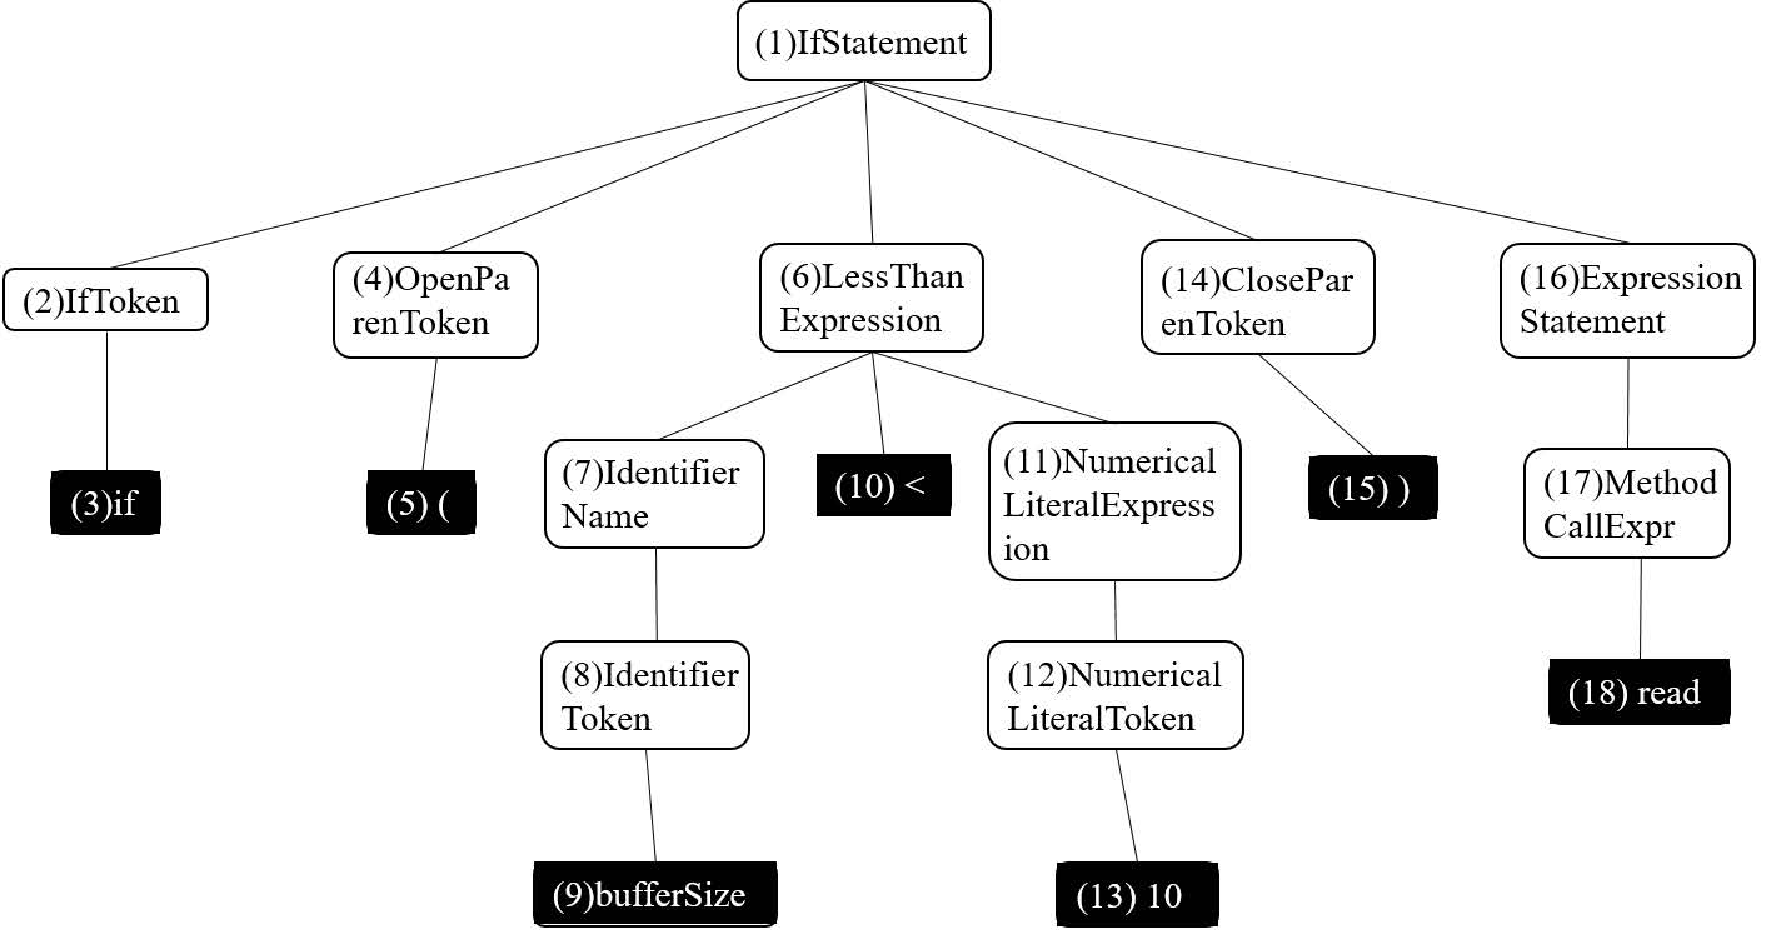
\includegraphics[width=15cm]{img/parseTree1.pdf}
 \caption{original parse tree}
\end{figure*}

\subsubsection{Our Parse Tree}\label{sec:ourParseTree}
Comparing to Fig.1 and Fig.2, there are many new internal nodes appears in the parse tree. These internal nodes are specific to programming language and the expression or statement that the source code is. So internal nodes hold much structural information. And the leaf nodes of parse tree are all appeared in the string of source code, they are all separated from the sequence of tokens.

But this kind of parse tree isn't fit for source code repositories very much. In source code repositories, most functions will call other functions to achieve their goals. If we want to know the subject of one function we must know the subject of functions that are called by this function. For example, we have a source code function is shown in Fig.4. When we want to know the subject of function getBufferSize, we have to know the subject of function read firstly. Because of this relation among functions, we add the functions's call graph into our parse tree. This means we replace the function's name in parse tree to the subject of function. Like word embedding, we represent the subject of function as a vector. And this subject vector is calculated from the parse tree of the called function(like read() function).

At the same time, we also found that in Fig.2, the node 10 is bufferSize, but bufferSize isn't a correct English word it is combined by buffer and size. If we use bufferSize directly, we may can't catch the subject of function exactly. So we split bufferSize into buffer and size, and add a new internal node called CombineName. This new internal node means there is identifier and this identifier is combined by the children of CombineName node.

After adding the call graph of functions and the new internal node(CombineName), the new parse tree of Fig.1 can be seen in Fig.3.
\begin{figure*}[!htp]
 \centering
 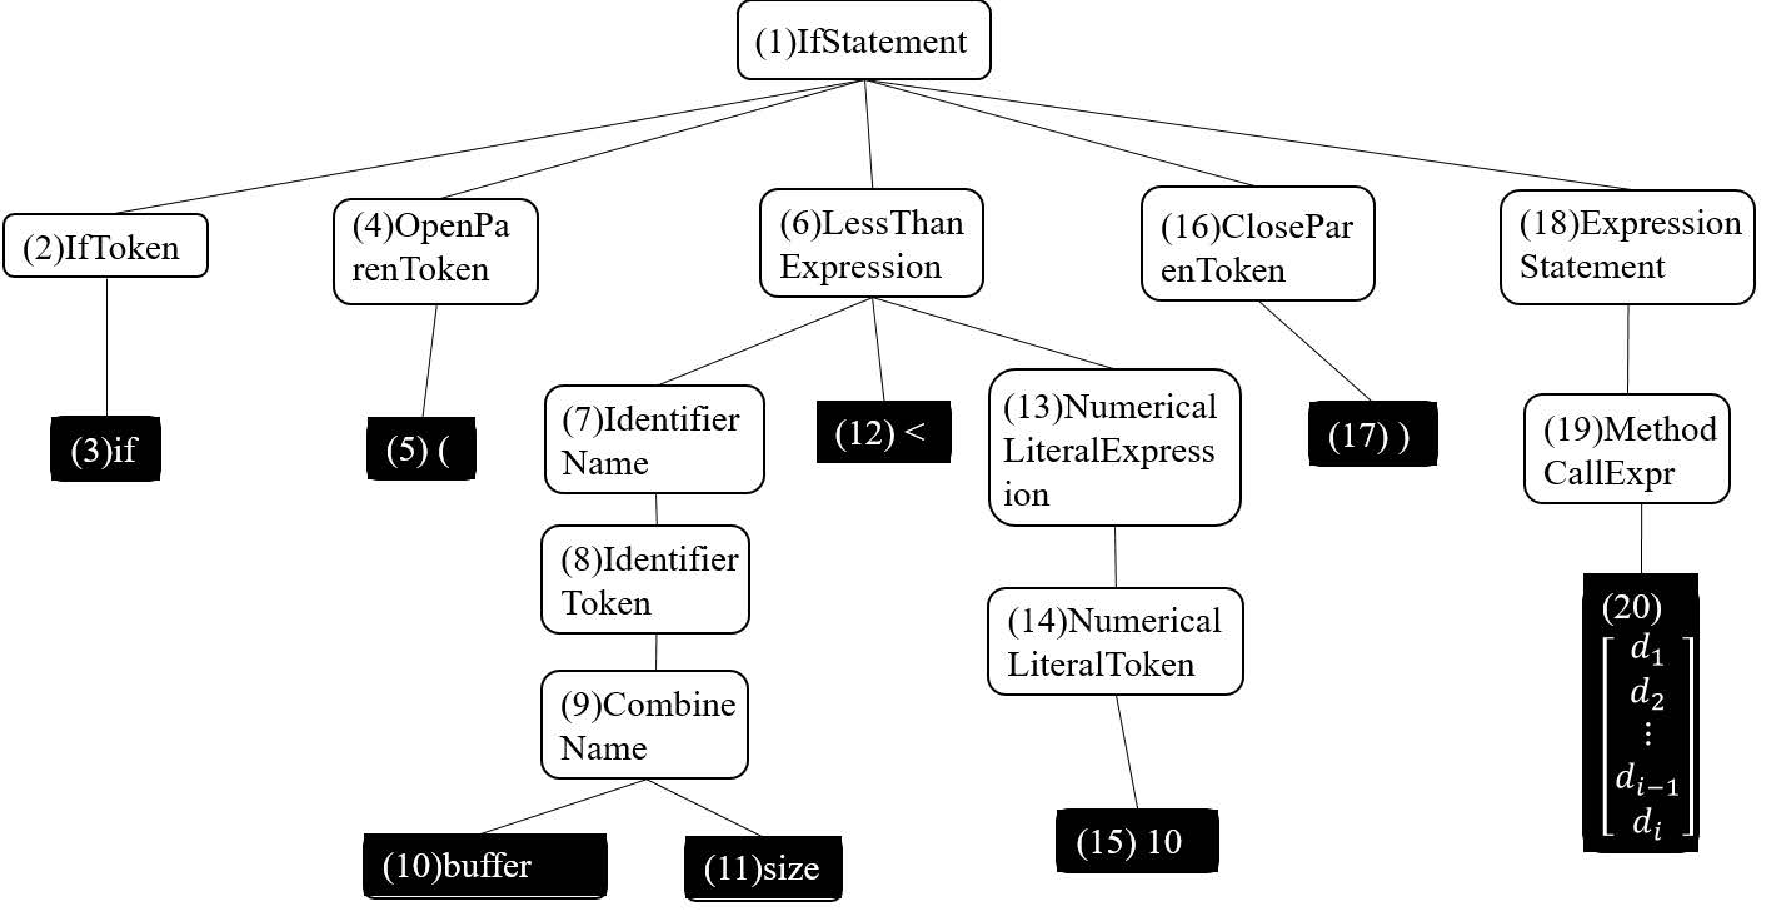
\includegraphics[width=15cm]{img/parseTree2.pdf}
 \caption{new parse tree}
\end{figure*}

\begin{figure}[!htp]

 $~~~~~~~~~~~~~$   int getBufferSize(int bufferSize)\{\\
 $~~~~~~~~~~~~~$  $~~~~$   if (bufferSize $>$ 0)\\
 $~~~~~~~~~~~~~$  $~~~~~~~~$     return read();\\
 $~~~~~~~~~~~~~$  $~~~~$    else\\
 $~~~~~~~~~~~~~$  $~~~~~~~~$      return 0;\\
 $~~~~~~~~~~~~~~$   \}
    \caption{function example}
\end{figure}

\begin{table}[!htp]\label{table:splitID}
\centering
\begin{tabular}{|c|c|}
\hline
Identifier & Words \\
\hline
contextInitialize & context, initialize\\
\hline
apiSettings & api, settings\\
\hline
buildDataDictionary & build, data, dictionary\\
\hline
add\_result & add, result\\
\hline
\end{tabular}
\caption{Example of Split Identifiers}
\end{table}

\begin{table}[!htp]\label{table:abbr}
\centering
\begin{tabular}{|c|c|c|}
\hline
Abbreviation & Origin & Context\\
\hline
val & value & key.value()\\
\hline
cm & confusion, matrix & new ConfusionMatrix()\\
\hline
conf & configuration & context.getConfiguration()\\
\hline
rnd & random & RandomUtils.getRandom()\\
\hline
\end{tabular}
\caption{Example of Split Identifiers}
\end{table}

\subsubsection{Identifier Operation}
According to the description in last section, some names of identifiers are phrases, which are meaningless since they are combined by
two or more meaningful words together. They are quite important since they are the semantic information in this parse tree, showing the objective of why
they are creative or what problems they solve. So we want to utilize such kind of information, instead of just keep the combination of them which makes no
sense. There are two kinds of method to improve the semantic information. One is to split all the phrases to multiple words and the other one is to retrieve the
full version from some abbreviated parameters.

From table 1, we see some examples of identifiers in source code. They are defined in the combination of some words, using the alternation of capital and small
letters or splitting two words with a underscore. For example, when we name a parameter whose function is to add two integers, we can name it as ``addScore'',
changing the first letter of the second word to a capital one. When we encounter an identifier, we can search the alternation of capital and small letters, or
observe the appearance of underscores.

Another situation is that many identifiers are also meaningless since they are the abbreviation of one or more words. Table 2 shows some abbreviations and
their original version. However, we can get their full name by checking their context. As we observed, we can split the context to words. Then, check the
initials of these words to see whether they make up of the identifier we are operating. Take ``cm'' in table 2 as an example. When searching its context we can
find ``confusion'' and ``matrix'', whose initials can make up of ``cm''. So we can believe the full version of ``cm'' is ``confusion matrix''.

When parsing the code, adding such two kinds of operations can add more semantic information into the parse tree, which serves the goal that combining
semantic and structural information together.

\subsection{Bimodal Modelling of Source Code and Natural Language}
We joint source code functions and tags with the model mentioned in [1]. Miltiadis's model can be used to match source code snippets and natural language query. But the code snippets in [1] must has less than 300 words, while there are many functions that have more than 300 words in our model. And natural language query is also different from the tag. In our model, tags are many individual words and don't have any relationship with each other while training. But the words in the same query sentence must be trained together.

So we change some aspects of [1] to make our model more suit to code repository and the new parse tree is one of changes.
\subsubsection{Notation}
We let $I$ be the set of internal nodes and $K$ be the set of leaf nodes. And a parse tree can be represented as $C\ =\ (Nd,ch,val)$ where $Nd=\{1,2,\cdots,N\}$ is set of all nodes($Nd=I\cup K$) and $ch$ is a function that map the node to its children nodes. The last one $val$ is a function that match the index of node and the value of this node. For example, i is the index of node "read", then val(i) equals to "read". By the way, we index the nodes of parse tree by left-to-right depth first traversal of tree. Fig.2 and Fig.3 have shown some indexing examples.
\subsubsection{Model Overview}
We use a generative model to train our data. $P(C\ |\ T)$ is the probability of generating parse tree C based on the the tag T. And our goal is to maximum this probability.
\begin{align}
    P(C\ |\ T) & = \prod_{n\in Nd:ch(n)\neq\phi}^N P(val(ch(n))\ |\ T,C_{\leq n})
\end{align}
Equation(1) tells us how to calculate $P(C\ |\ T)$, and it means if we want to generate a parse tree C based on tag T, we have to sequentially generate a child tuple for node n conditional upon the tag T and the partial tree $C_{\leq n}$.

We also define $supp(i)$ and $S_{\theta}(v,T,C_{\leq n})$ like [?] to construct our model. $supp(i) = \{v\ :\ v=val(ch(n)) \bigwedge val(n)=i\ for\ some\ n\ in\ dataset\}$ is the set of all children tuples that appear as the children of a node whose type is $i$. And we can convert scoring function $S_{\theta}(v,T,C_{\leq n})$ to probability by exponentiating and normalizing.
\begin{align}
    P(v\ |\ T,C_{\leq n}) & = \frac{\exp s_{\theta}(v,T,C_{\leq n})}{\sum_{v^{'}\in supp(val(n))}\exp s_{\theta}(v^{'},T,C_{\leq n})}
\end{align}
where $\theta$ is the parameter of our model.
\subsubsection{Scoring Function}
The scoring function in our model is $s(v,T,C_{\leq n}) = (t \bigodot c)^{\top} r + b$ and $\bigodot$ is elementwise multiplication. $t$ is the representation vector of tag and c is the feature nodes' vector in the function's parse tree. $r$ is the vector that is unique to each parent-children pair $(i,v)$. $b$ is also unique to each parent-children pair, but $b$ is a scalar number.
\subsubsection{Training}
Our aim is to maximum $P(C\ |\ T)$, and because normalizing cost much time, we use noise-contrastive estimation method to train our model which is the same as [1]. The objective function can be written as follows:
\begin{align}
  \nonumber  E_{(T,C_{\leq n},v)\sim D}[\log\Delta(\triangle s(v,T,C_{\leq n}))]\ +\ \\ kE_{(T,C_{\leq n},v^{'})\sim noise}[\log(1-\Delta(\triangle s(v^{'},T,C_{\leq n})))]
\end{align}
where $d$ is the distribution of data and $nosie$ is the distribution of the noise data. The noise data's distribution is the posterior PCFG of the training data. And $k$ means that every pair $(T,C_{\leq n})$ has $k$ noise data. And we choose the same initialization strategy as [1] says.
